\begin{figure}[ht!]
\centering
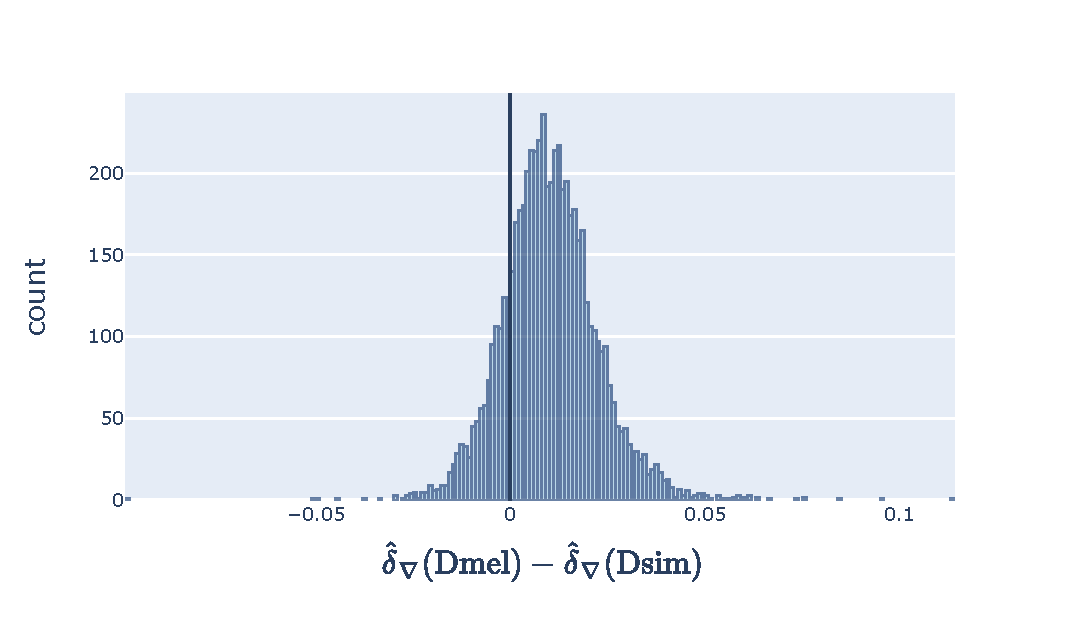
\includegraphics[width=	\textwidth]{figures/plots/drosophila/d-conv-diff.pdf}
\caption[The magnitude of mutation disequilibrium is higher in \textit{D. melanogaster} than in \textit{D. simulans}]{\textbf{The magnitude of mutation disequilibrium is higher in \textit{D. melanogaster} than in \textit{D. simulans}}. Each data point in the distributions are the difference between a gene in \textit{D. melanogaster} and in its ortholog in \textit{D. simulans} for \textbf{(a)}, ENS, and \textbf{(b)}, $\hat\delta_\nabla$ . 75\% of genes had higher ENS in \textit{D. melanogaster}. 82\% of genes had a higher $\delta_\nabla$ in \textit{D. melanogaster}. Data included from $\sim 5,900$ CDS alignments of \textit{D. melanogaster}, \textit{D. simulans} and \textit{D. yakubra}. The CDS sequence of the gene is third codon position only.}
\label{fig:drosophila_d-conv-diff}
\end{figure}
